\section {Introduction}

Many of the searches for \charginopm and \neutralinotwo in ATLAS \cite{Aad:2012hba, ATLAS:2012ab} and CMS \cite{Chatrchyan:2012mea} involves the search for signal events with 3 leptons and \met. On the other hand there are very few searches involving final states with $\tau$ leptons due to the the larger $\tau$ misidentification rate which makes harder to keep the background under control as well as having low \pt thresholds for triggering.

\begin{figure}[tbh!]
	\centering
	\begin{tabular}{cc}
		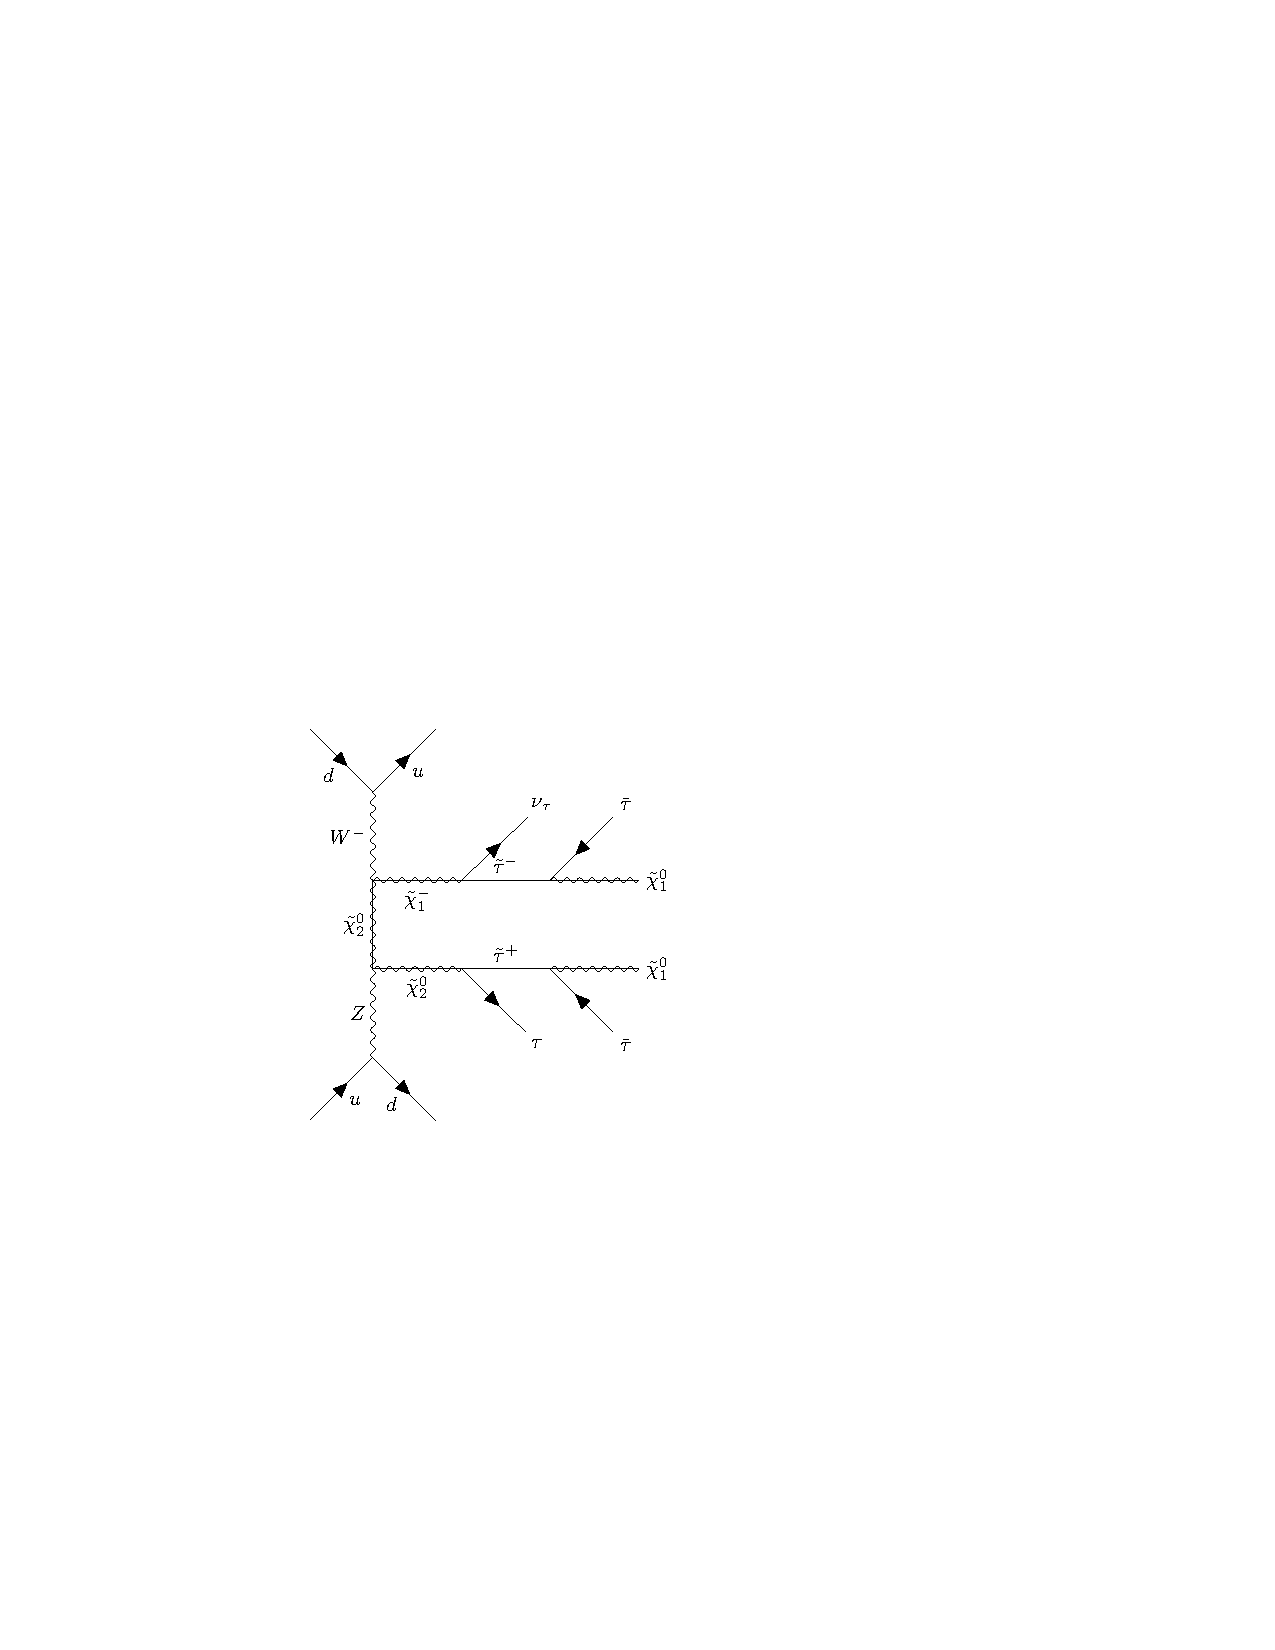
\includegraphics[width=0.48\textwidth]{diagrams/pics/signal_C1N2.pdf}
		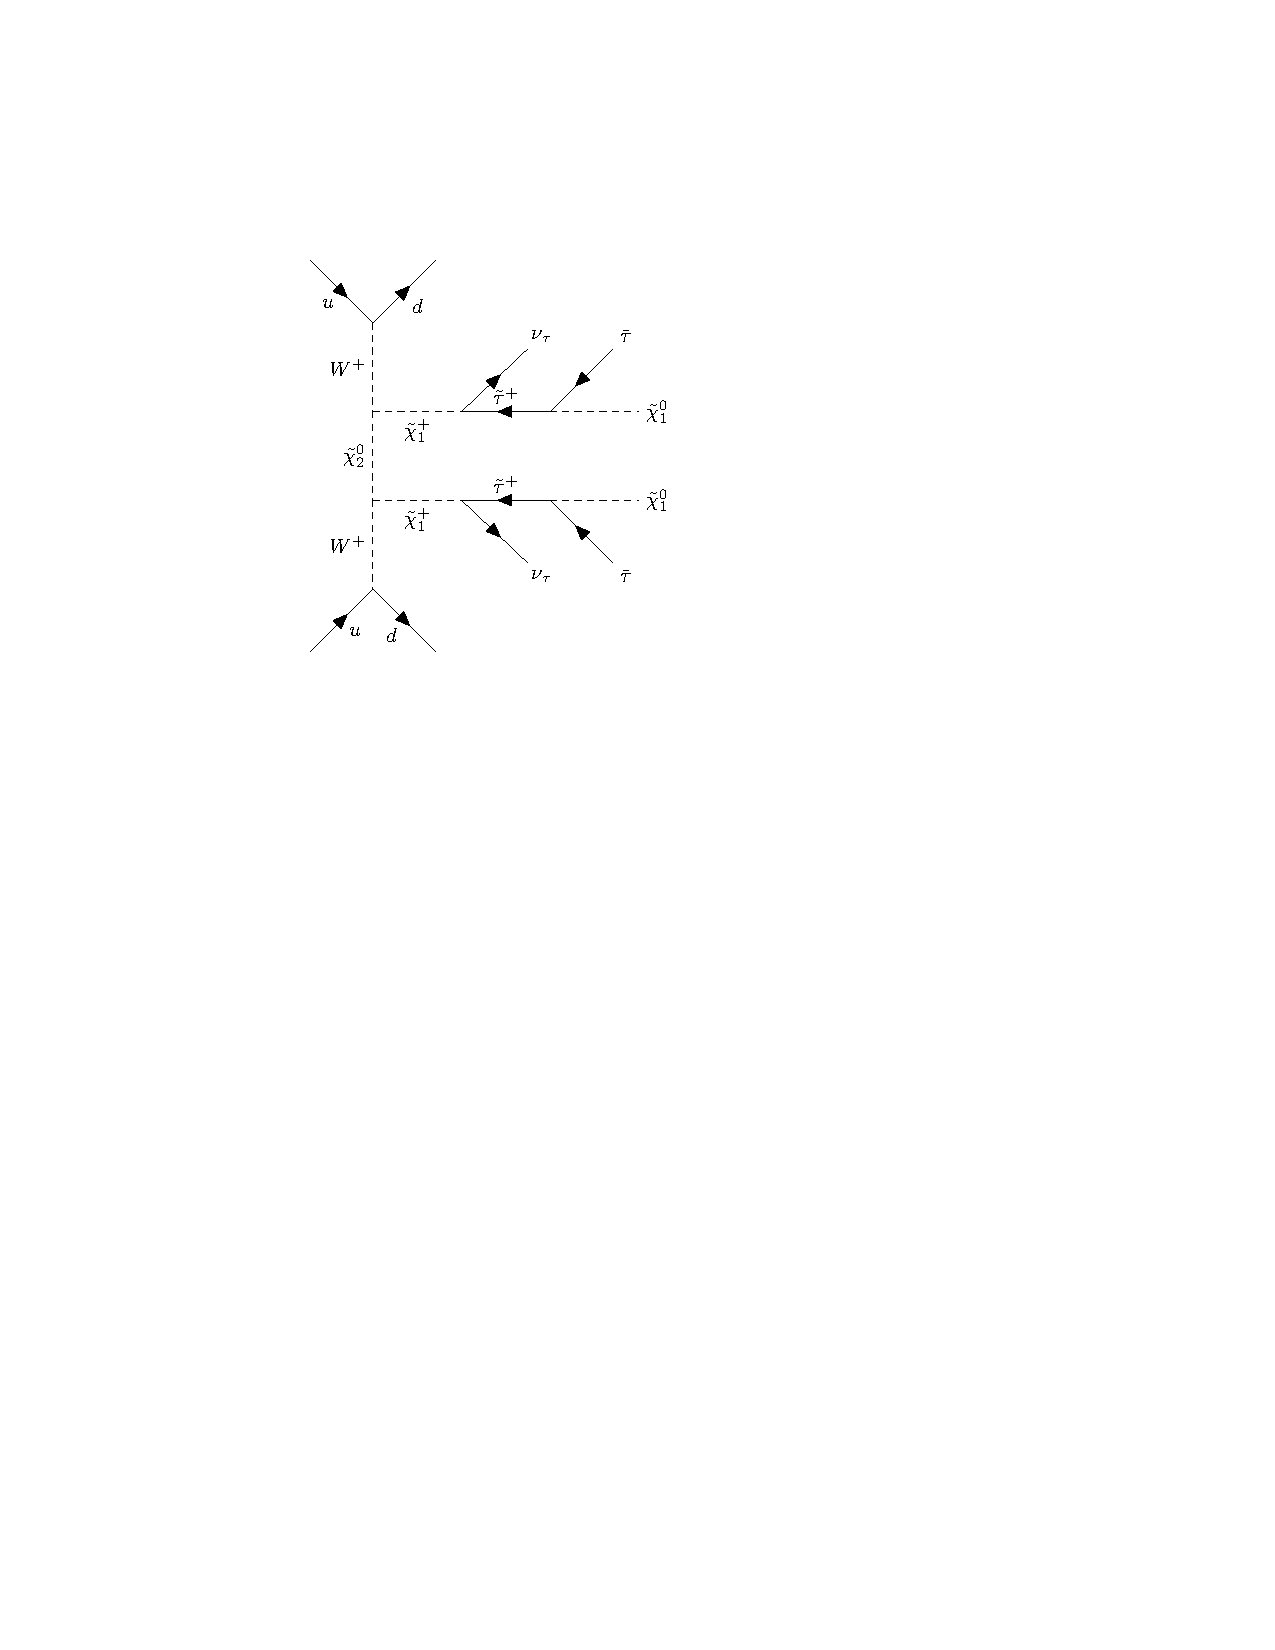
\includegraphics[width=0.48\textwidth]{diagrams/pics/signal_C1C1.pdf} 		
	\end{tabular}
	\caption{Diagrams of (left) \charginopm \neutralinotwo and (right) \charginopm \charginomp pair production through vector-boson fusion followed by their decays to $\tau$ leptons and the LSP.}
	\label{fig:VBF_diagrams}
\end{figure}

Early studies on the kinematics of Vector Boson Fusion (VBF) processes suggest the possibility for the analysis of the \charginopm / \neutralinotwo system \cite{Bjorken:1992er}. VBF production is characterized by the presence of two jets with large di-jet invariant mass in the forward region in opposite hemispheres. Additionally the \charginopm and \neutralinotwo decays into multiple $\tau$ leptons and \neutralinoone which travels through the detector undetected increasing \met. A sample diagram of \charginopm / \neutralinotwo pair production from VBF processes is shown in Figure \ref{fig:VBF_diagrams}. This search comes with some important advantages \cite{Dutta:2012xe}.

\section {Search Strategy}
\label{section::search_strategy}

For this type of search several benchmark points are defined under the following constraints. Firstly the \charginopm and \neutralinotwo are mainly Wino-like, while the \neutralinoone is mainly Bino-like. Furthermore the \charginomp mass similar to the \neutralinotwo mass ($m_{\charginopm} \sim m_{\neutralinotwo}$) and with values of 100, 200 and 300\gev. Additionally the mass gap between the \stau and \charginopm is either 5 \gev or $(m_{\stau} - m_{\charginopm})/2$. Finally The LSP mass is either $\neutralinoone = 0$, or 50\gev.

The processes taken into account are

\begin{equation}
pp \longrightarrow \charginopm \charginomp jj, \quad pp \longrightarrow \charginopm \neutralinotwo jj, \quad pp \longrightarrow \neutralinotwo \neutralinotwo jj
\end{equation}

The cross-section prediction for each of those processes are shown in Figure \ref{fig:VBF_xsec} as function of the \charginomp - \neutralinotwo mass.

\begin{figure}[tbh!]
	\centering
	\begin{tabular}{cc}
		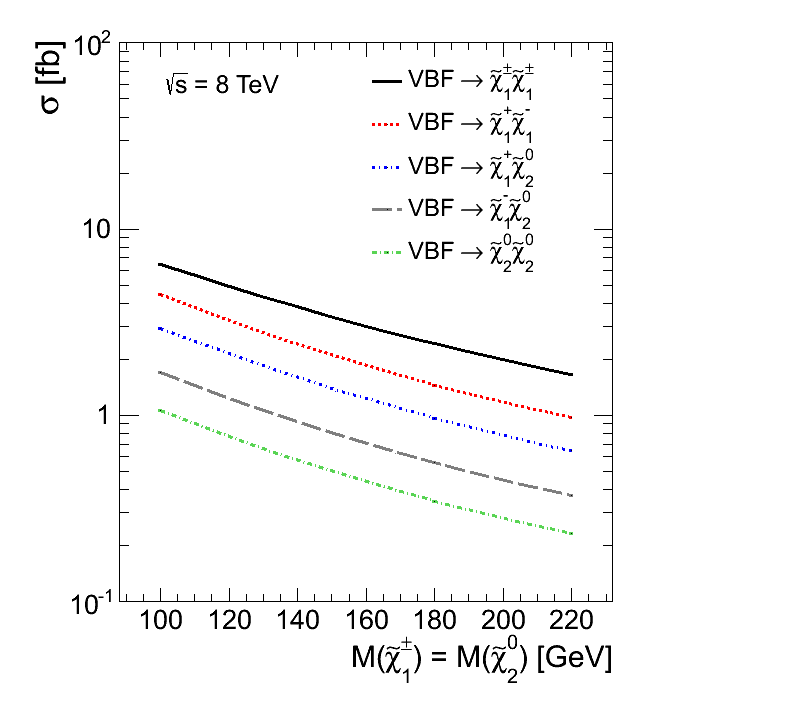
\includegraphics[width=0.75\textwidth]{analysis/pics/VBFXsection.png}
	\end{tabular}
	\caption{VBF production cross-section at \CM = 8 \tev as a function of mass for various channels after imposing \ensuremath{\deltaeta > 4.2} using Madgraph 4 \cite{Dutta:2012xe}.}
	\label{fig:VBF_xsec}
\end{figure}

The search strategy can be divided in two distinct parts: the first one considers the kinematic of the jets produced via VBF in order to reduce the contribution coming  from V + jets events (where V is ether the W or Z boson); the second one takes into account decay products of the supersymmetric particles falling into the inner region of the detector (centrally produced) in order to reduce the all the non-supersymmetric background contributions.

\begin{figure}[tbh!]
	\centering
	\begin{tabular}{cc}
		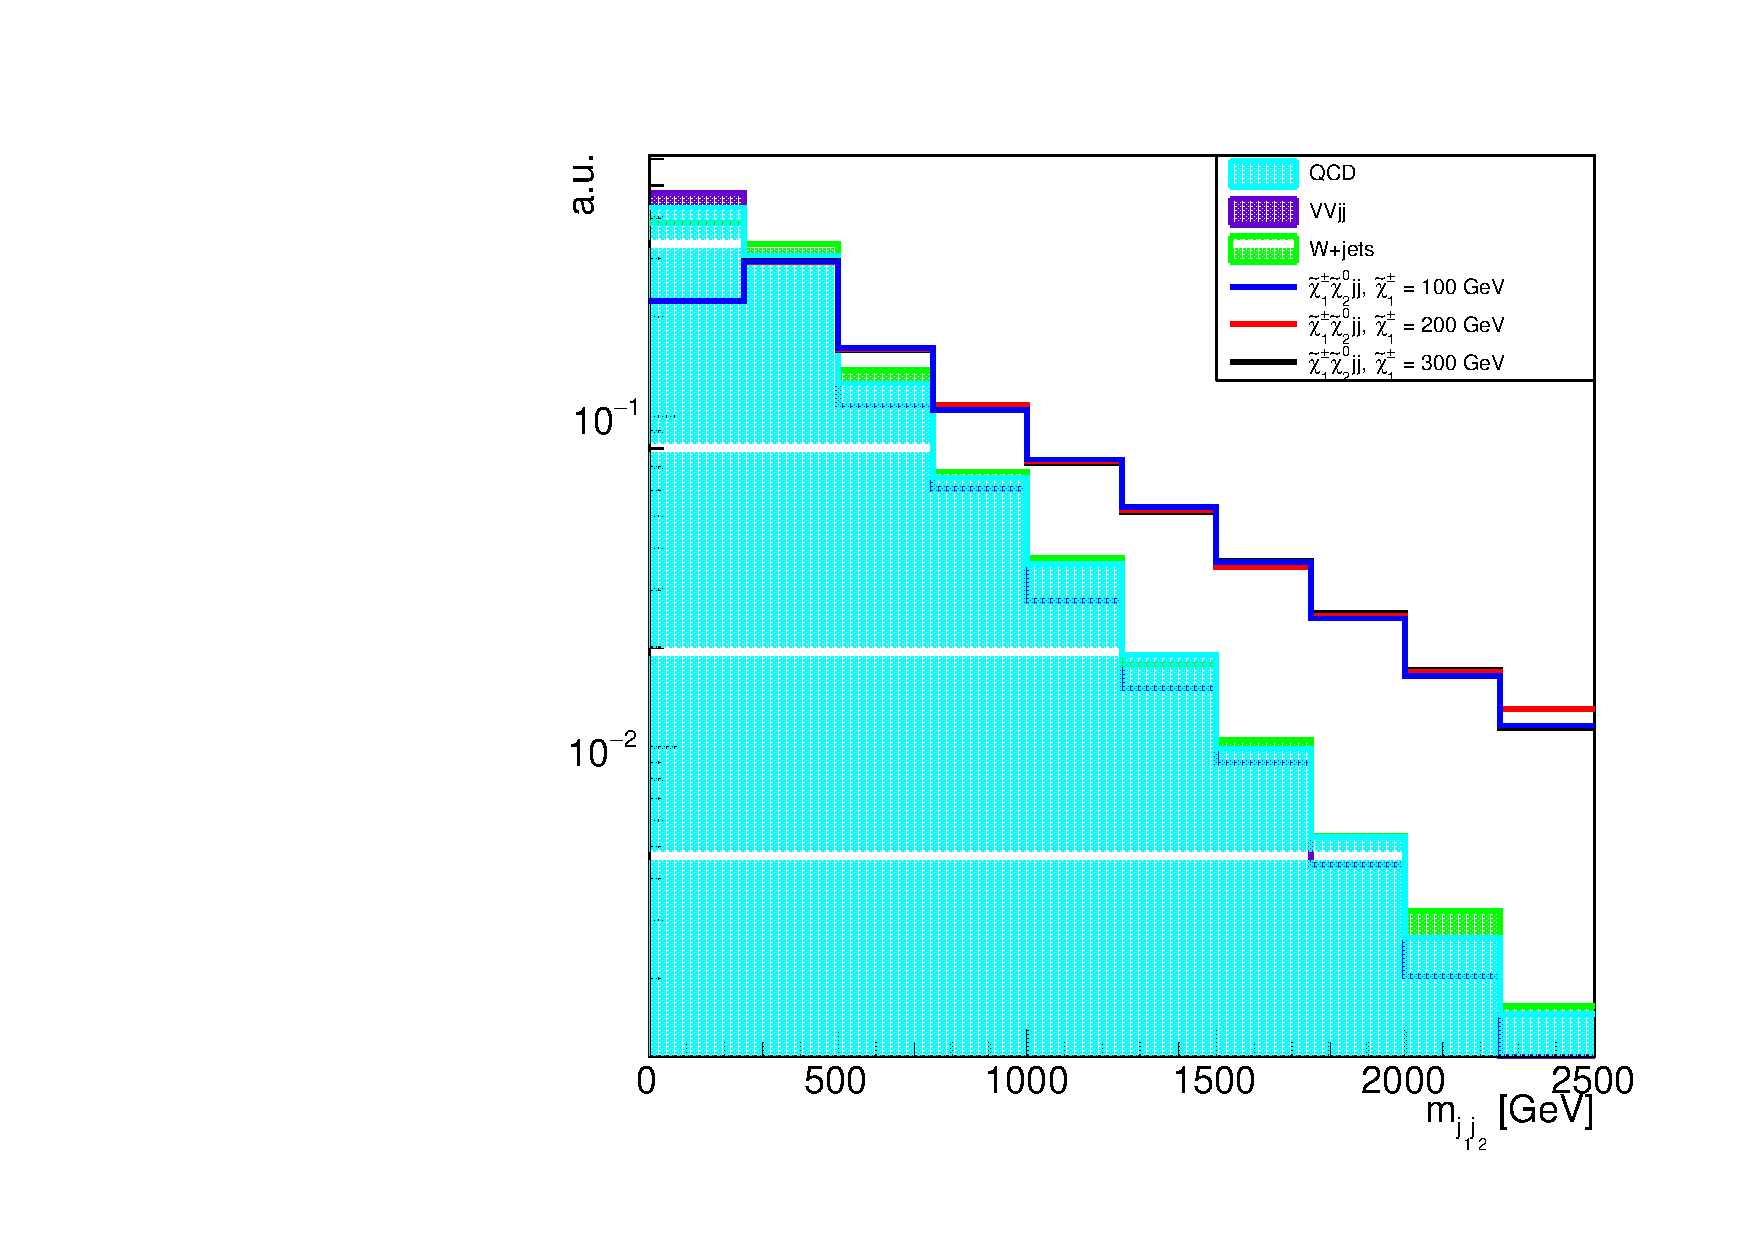
\includegraphics[width=0.48\textwidth]{analysis/pics/h_dijetinvariantmass_prospects13tev.pdf}
		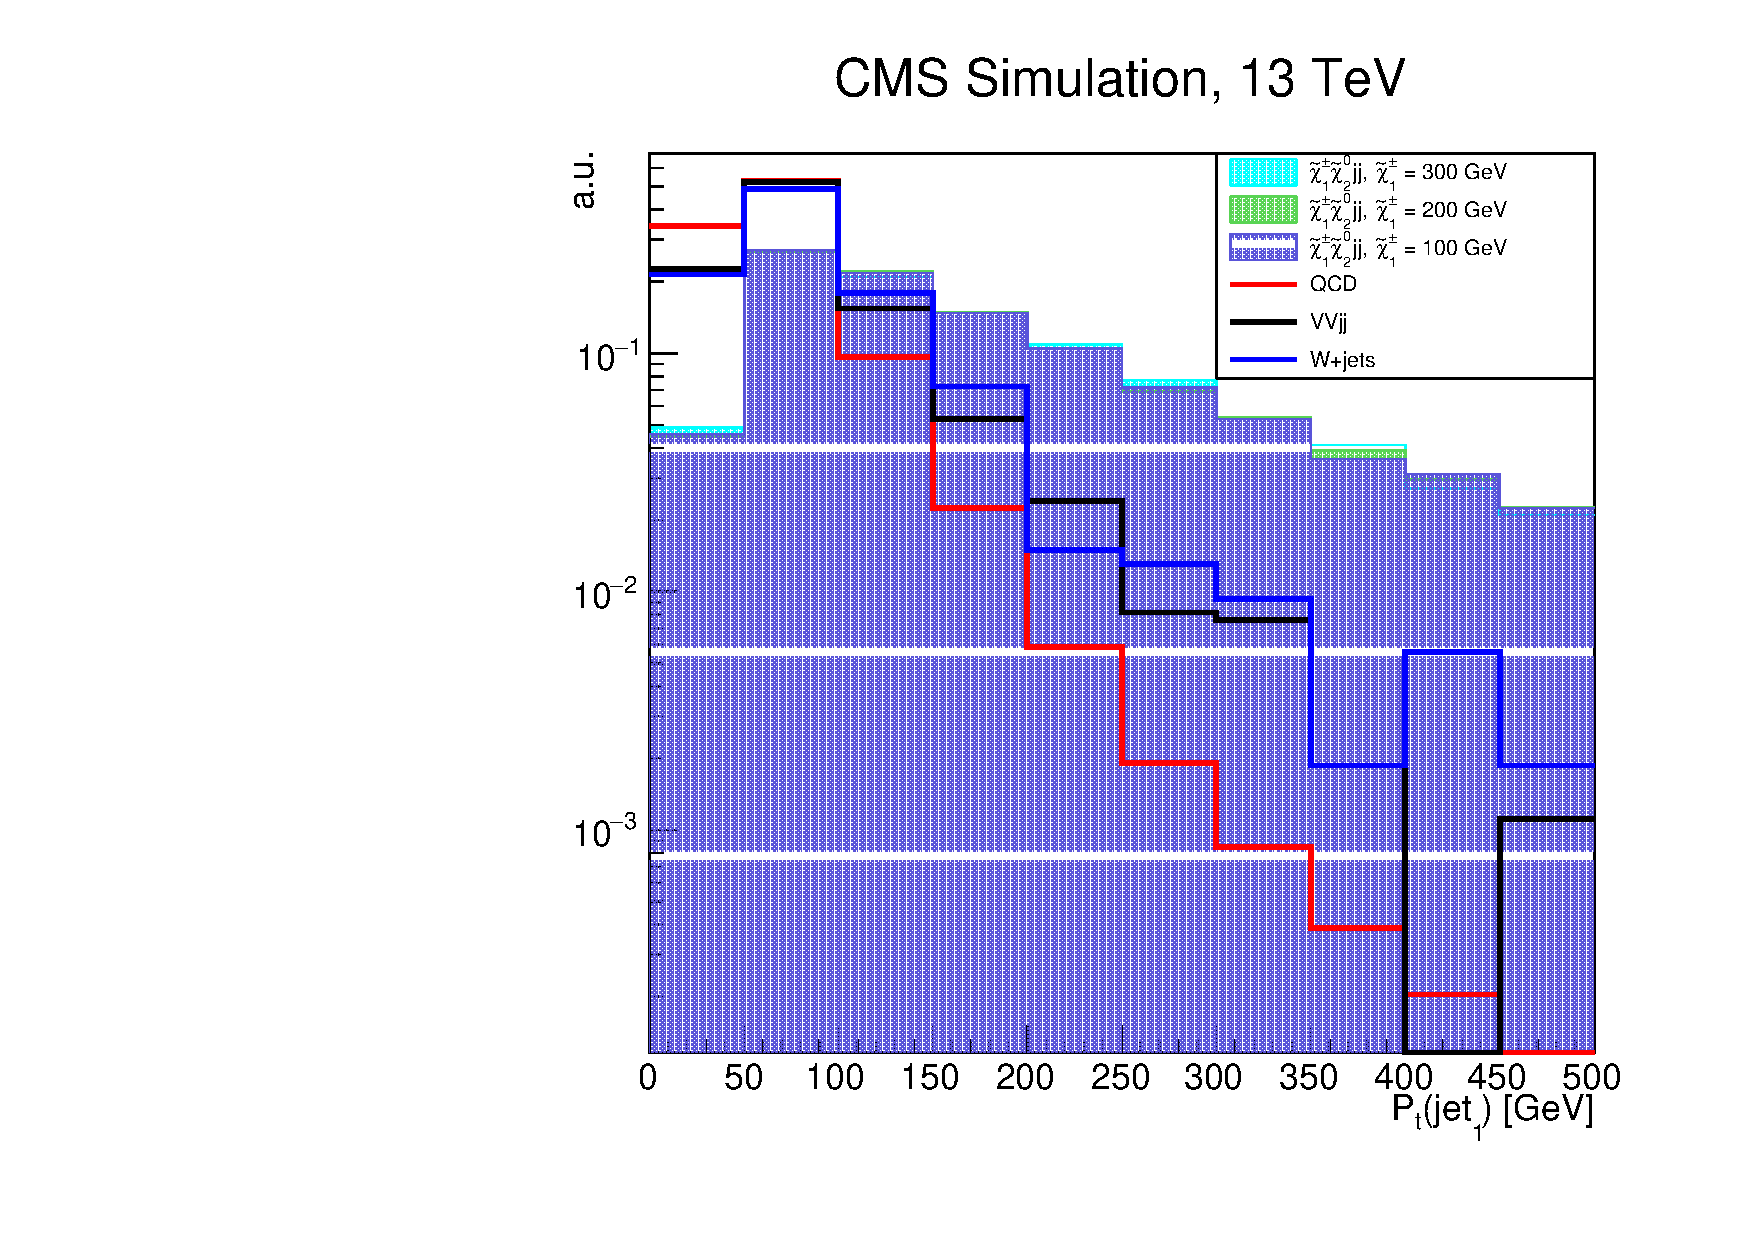
\includegraphics[width=0.48\textwidth]{analysis/pics/h_jet1pt_prospects13tev.pdf} 		
	\end{tabular}
	\caption{\ensuremath{m_{j_{1}j_{2}}} (left) and \pt of the leading jet (right) distributions normalized to arbitrary units for \charginopm \charginopm pair production by VBF processes, V+jets background, and VV background produced by VBF processes and QCD processes. The chosen signal benchmark point features \ensuremath{m_{\charginopm} = m_{\neutralinotwo} = 300, 200 and 100\gev}, \ensuremath{m_{\charginopm} - m_{\tilde{\tau}} = 5\gev} and \ensuremath{m_{\neutralinoone} = 0\gev}.}
	\label{fig:VBF_mjj_ptj1}
\end{figure}

\begin{figure}[tbh!]
	\centering
	\begin{tabular}{cc}
		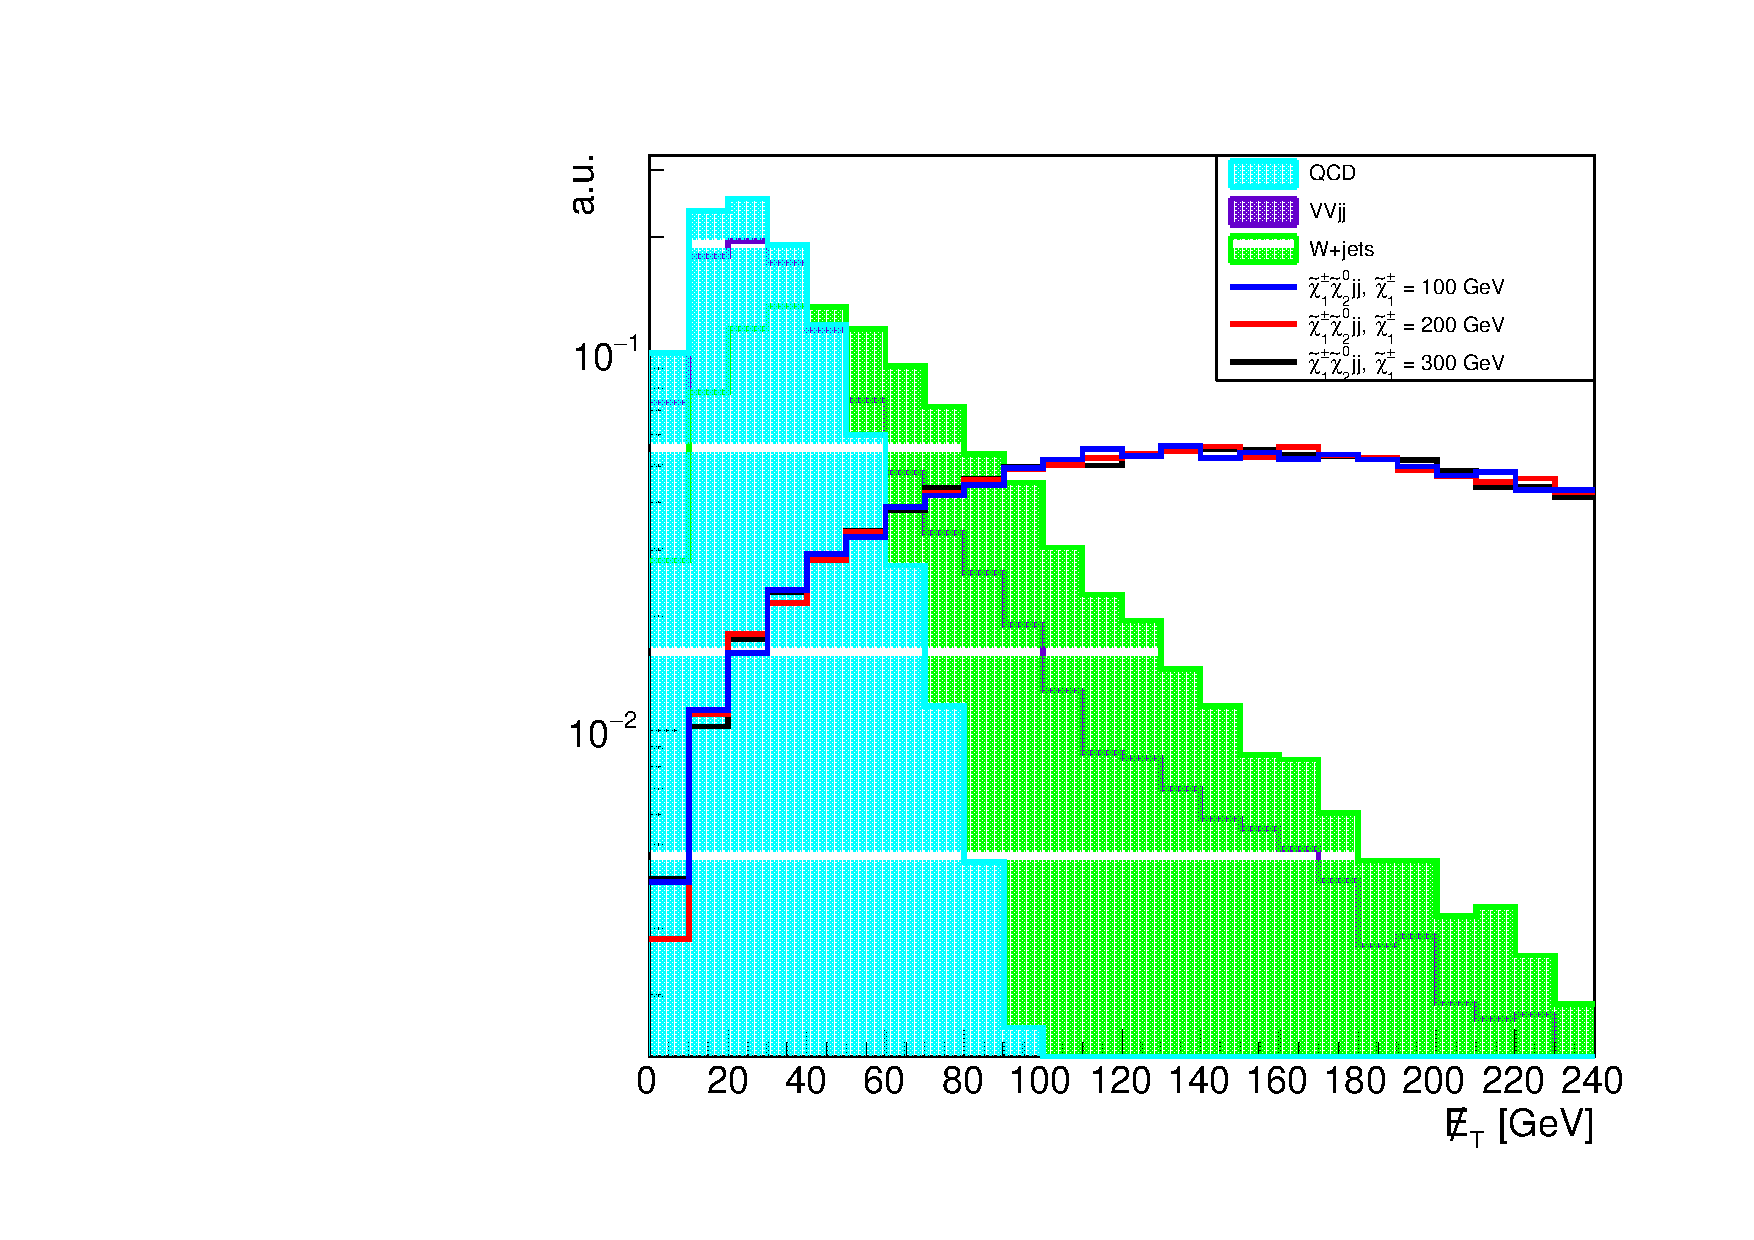
\includegraphics[width=0.48\textwidth]{analysis/pics/h_met_prospects13tev.pdf}
		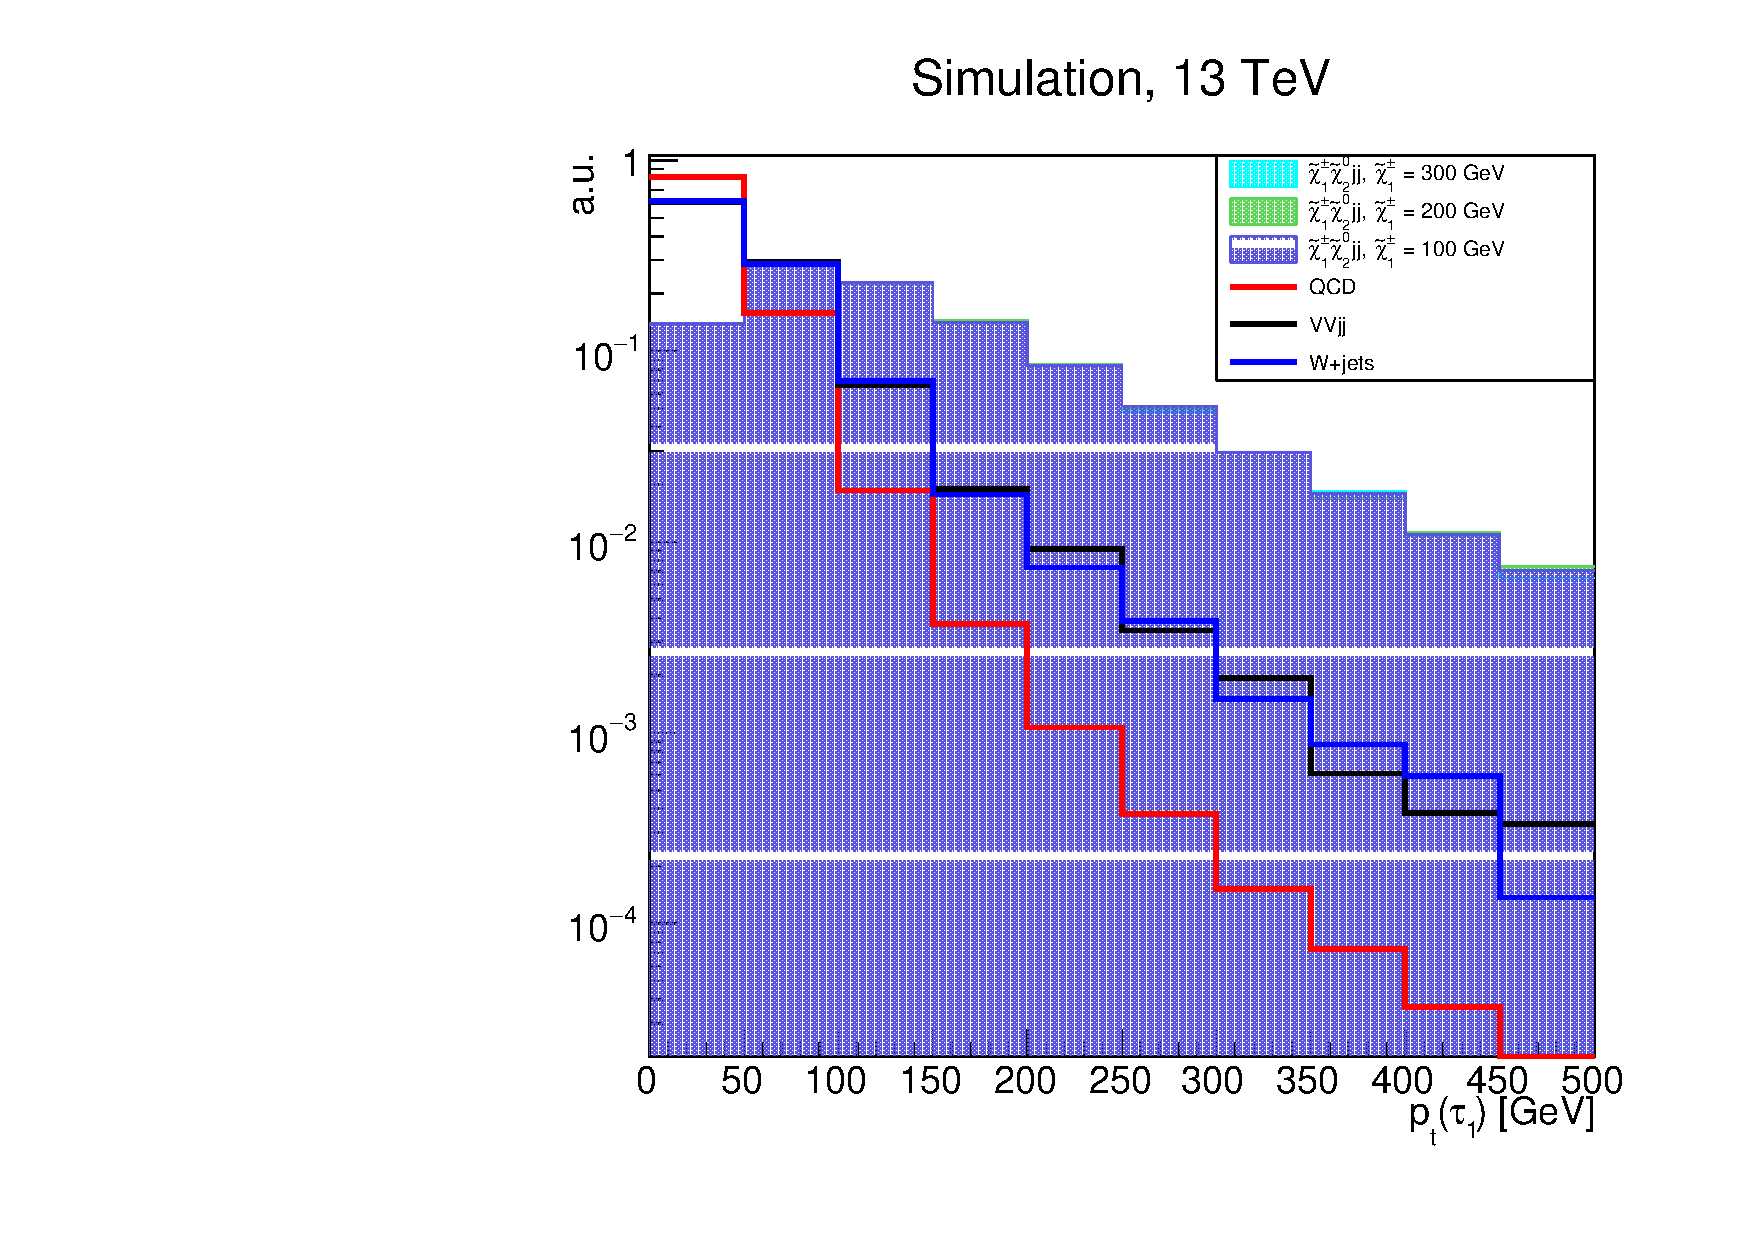
\includegraphics[width=0.48\textwidth]{analysis/pics/h_tau1pt_prospects13tev.pdf} 		
	\end{tabular}
	\caption{(left) \met and (right) leading \ensuremath{\tau} \pt distributions normalized to arbitrary units in \ensuremath{\geq 2j + 2\tau} final state for \charginopm \charginopm pair production by VBF processes, V+jets background, and VV background produced by VBF processes and QCD processes. The chosen signal benchmark point features \ensuremath{m_{\charginopm} = m_{\neutralinotwo} = 300, 200 and 100\gev}, \ensuremath{m_{\charginopm} - m_{\tilde{\tau}} = 5\gev} and \ensuremath{m_{\neutralinoone} = 0\gev}.}
	\label{fig:VBF_met_pttau}
\end{figure}

\section{VBF with two leptons and two jets}

Firstly with the increasing LHC luminosity both ATLAS and CMS needs to raise the \pt thresholds on the triggered objects with a consequent lowering of signal efficiency.  Is it possible however to probe signal for SUSY by triggering over the VBF properties of the event, leaving the decay products of \charginopm and \neutralinotwo free from online kinematic constraints.

Secondly VBF production allows the investigation of final states with $\tau$. \stau is typically lighter than \smuon and \selectron for large \tanbeta \cite{Hinchliffe:1999zc}. A light \stau with small mass splitting is favored in coannihilation processes \cite{Griest:1990kh} that set the relic density to correct values, in the case of Bino dark matter. Light \stau is also motivated in the context of the MSSM by the enhancement of the $H \longrightarrow \gamma\gamma$ channel \cite{Carena:2011aa}. These facts stress the importance of searches in $\tau$ final states with low \pt and large backgrounds, for which production by VBF processes is more suited since the VBF signature allows for the reduction of the backgrounds to manageable levels.

As third and final reason Drell-Yan production cross-section falls faster than the VBF production cross-section with increasing mass \cite{Datta:2002vy} allowing further control over background distributions.

The main feature of VBF processes is the production of a jets pair aimed at the forward-backward region of the detector with high \pt and large \deltaeta. By adding to the event selection the requirements on the di-jet \deltaeta as well as the di-jet invariant mass \ensuremath{m_{j_{1}j_{2}}} the background contribution coming from V+jets and \ttbar events, shown in Figures \ref{fig:background_W3jets} and \ref{fig:background_ttbar}, is kept under control. In order to generate super-symmetric particles, the incoming partons need to have an high momentum, therefore the leading jet from the VBF-produced di-jet pair is expected to have high \pt. The addition of a \pt cut on leading jets keeps further reduces background contributions. Figure \ref{fig:VBF_mjj_ptj1} shows a study on \ensuremath{m_{j_{1}j_{2}}} and leading jet \pt distributions for \charginopm \charginopm pair production by VBF processes, V+jets background, and VV background produced by VBF processes for \ensuremath{m_{\charginopm} = m_{\neutralinotwo} = 300, 200 and 100\gev}, \ensuremath{m_{\charginopm} - m_{\tilde{\tau}} = 5\gev} and \ensuremath{m_{\neutralinoone} = 0\gev}.

The remaining background contributions come from all the centrally produced particles. By considering an R-parity conserving model the decay of \charginopm and \neutralinotwo is the following

\begin{equation}
\charginopm \longrightarrow \stau^{\pm} \nu \longrightarrow \tau^{\pm} \neutralinoone \nu
\end{equation}

\begin{equation}
\neutralinotwo \longrightarrow \stau^{\pm} \tau^{\mp} \longrightarrow \tau^{\pm} \tau^{\mp} \neutralinoone
\end{equation}

The processes that have the same signature as signal are all the VV (where V may be wither W or Z) pairs produced via VBF where the bosons decays leptonically. Furthermore in case of \hadtau decays Quantum Chromo Dynamics (QCD) multijet becomes the most appreciable background contribution. A \met cut is effective in reducing those backgrounds as shown on Figure \ref{fig:VBF_met_pttau}. Moreover, requiring multiple $\tau$’s in the event further reduces background. The \pt of the \ensuremath{\tau} coming from the \charginopm and \neutralinotwo decays is strongly correlated to the mass difference between the \charginopm and the \neutralinoone LSP. In Figure \ref{fig:VBF_met_pttau}, the normalized distribution of the \pt of \ensuremath{\tau} is displayed for \ensuremath{m_{\charginopm} = m_{\neutralinotwo} = 300\gev}, \ensuremath{m_{\charginopm} - m_{\tilde{\tau}} = 5\gev} and \ensuremath{m_{\neutralinoone} = 0\gev}. For smaller \ensuremath{\Delta M}, the distribution peaks at lower \pt and the signal acceptance is less efficient.

\section{VBF with two hadronic $\tau$ and two jets}

Besides the two oppositely directed forward jets that define the VBF configuration, the search requires the presence of at least two leptons coming from the different decay modes of the $\tau$ and large \met. The chosen search channels are $e\mu jj$, $\mu\mu jj$, $\mu\hadtau jj$, and $\hadtau\hadtau jj$. The final states are further differentiated into like-sign (LS) and opposite-sign (OS) di-lepton pairs for a total of eight different search channels. This thesis focuses its attention on the di-\hadtau LS channel search and its background estimation strategy. 

